% kapitel4.tex

\chapter{Preselection in the Boosted Channel}

\section{Event Preselection}
\label{Event Preselection}
The Monte-Carlo samples used in this analysis have a specific preselection.\\
In table \ref{Event preselection} the different requirements are listed, which are part of this preselection. 

\vspace{0.5cm}

\begin{table}
\centering
\setlength{\tabcolsep}{3cm}
\begin{tabular}{|c|} 
\hline
\textbf{Event preselection} \\
\hline
\hline
\vspace{-0.3cm}
\\
Z boson candidate preselection:\\
\vspace{-0.1cm}
\footnotesize{$\bullet$ pair of opposite sign leptons (same flavor)} \\

\footnotesize{$\bullet$ $\mid m_{l^{+} l^{-}} - m_{Z} \mid$ < \SI{10}{GeV}} \\
\\
\vspace{-0.9cm}
\\
\hline
\vspace{-0.3cm}
\\
$\geq 2$ central jets \\
\vspace{-0.4cm}
\\
$\geq$ 2 b-tags\\
\vspace{-0.4cm}
\\
= 2 leptons \\
\hline
\end{tabular}
\caption{Preselection criteria.}
\label{Event preselection}
\end{table}


The first aspect is the Z boson candidate preselection. 
According to the studied leptonic decay channel of the Z this includes a reconstructed Z candidate mass with \SI{10}{GeV} around the real Z pole resulting from two opposite sign leptons with same flavor.
In this analysis only electrons and muons are considered in the Z candidate reconstruction and not the $\tau$ lepton or neutrinos.
Figure \ref{Zmass} shows the distribution of the reconstructed Z mass. 
Both signal and background are presented in one plot and are normalized to unity. 
The background is illustrated as colour filled histogram with a specific colour for each background process which is listed in the legend.
The different background processes are stacked. 
The signal is shown as solid red and blue line for the BBS and TTS process.
In the legend the weighted number of events is displayed in brackets next to each process.
Furthermore the statistic errors are shown as vertical lines.
The shape of the distribution looks like expected because it displays a pole mass distribution which is smeared because of detector influences.
Processes including a real Z like the signal and Z+jets processes have a peak at the Z mass. 
The \ttbar{} background process has no peak at the Z pole mass which is as anticipated as well because the leptons result from W boson decays.\\
Furthermore in the preselection at least two central jets with $\mid\eta\mid < 2.5$ and $p_{T} < \SI{25}{GeV}$ are required.
These jets are called central jets.
The $p_{T}$ requirement should ensure that the jets are calibrated and the $\eta$-regio is limited because the detector resolution in this $\eta$-region is higher than in regions with $\mid \eta \mid > 2.5$.  
Because of the specific decay topology two or more b-tags for the central jets are expected.
One b-jet results straight from the vector-like quark decays T\texorpdfstring{$\longrightarrow$}~Wb and B \texorpdfstring{$\longrightarrow$}~Zb.
The other is caused by the third generation top quark decays t\texorpdfstring{$\longrightarrow$}~Wb.
The top quarks are the decay products of the second vector-like quarks with T\texorpdfstring{$\longrightarrow$}~Zt and B\texorpdfstring{$\longrightarrow$}~Wt.\\  
The last aspect of the preselection listed in table \ref{Event preselection}  is the requirement of exact two leptons. 
This should guarantee the analysis in the dileptonic channel. 

\begin{figure}
\centering
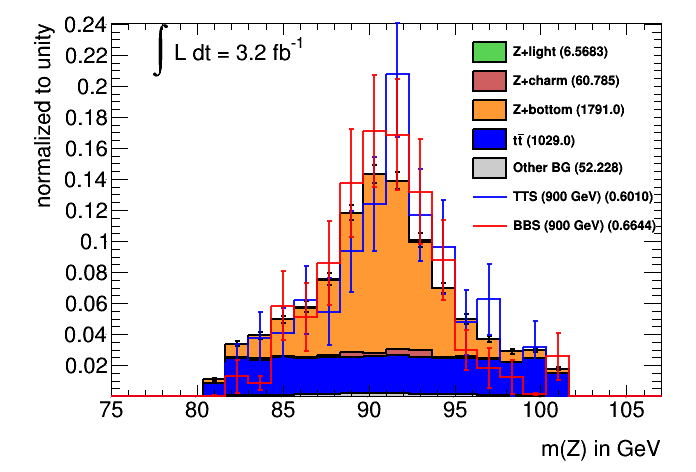
\includegraphics[width=11cm]{figures/Zmass.png}
\caption{Distribution for the reconstructed Z boson mass after the preselection.}
\label{Zmass}
\end{figure}

\section{Boosted Analysis Strategy}
The samples are simulated with a vektor-like quark mass of $m_{T/B} =$ \SI{900}{GeV}. 
Because of the massive vektor-like T and B the decay products have very high transverse momenta. 
Caused by the high transverse momenta the particles of the subsequent decays are strongly collimated. 
This situation is illustrated in figure \ref{boosted} for a top quark decay.
The figure shows the decay for a low and a high top $p_{T}$.
As mentioned before the figure shows that the decay products of the top are collimated for a high top $p_{T}$.\\
This collimated structure of the particles have an inpact on the clustering algorithms used in the ATLAS experiment.
Jets can for example be clustered with a anti-$k_{t}$ jet clustering algorithm \cite{antikt}.  
The anti-$k_{t}$ algorithm clusters soft particles around a hard particle within a given radius and forms conical jets. 
If two hard particles are located within an area closer than $\Delta R$ the clustering algorithm is not able to form a smooth circular shape around the hard particles.  
For a low top $p_{T}$ a $\Delta R = 0.4$ can be used.
In the high $p_{T}$ regions it is probable, that the jets from the top decay, which are clustered with $\Delta R = 0.4$  merge because the one decay product can be in an area $\Delta R$ around the other. 
Hence as mentioned before the anti-$k_{t}$ algorithm is not able to form smooth circular shapes. 
To avoid this problem the boosted analysis strategy can be used for high top transversal momenta.
The idea of the boosted analysis strategy is to cluster one jet which have all decay products of a boosted particle in it.
The area, where the decay products of a particle are located can be estimated with the formula $R \approx \frac{2m}{p_{T}}$ .
In the boosted analysis a radius of $\Delta R = 1.0$ for the cluster algorithm is used. 
A combined result from the top quark mass measurement is $m_{t} =$ \SI{173.29 \pm 0.95}{GeV} \cite{topmass}.
Using the formula mentioned before the boosted analysis is sensibel for a $p_{T}$ of the top quark about \SI{346}{GeV} and more. 
The boosted analysis strategy can be used for a boosted decay of a W boson, too.

\begin{figure}
\centering
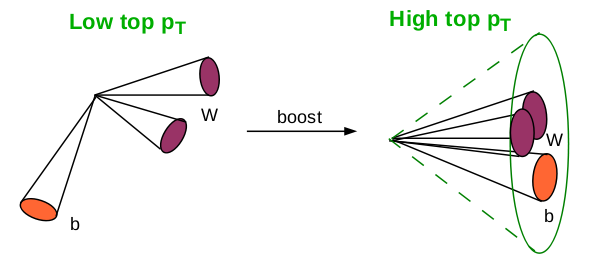
\includegraphics[width=11cm]{figures/boost.png}
\caption{Representative figure for a top quark decay with a high and a low top $p_{T}$ created by Emily Thompson.}
\label{boosted}
\end{figure}

In this analysis jets clustered with  $\Delta R = 1.0$ are used.   
These jets are called large-R jets. 
Large-R jets offer the possibility to introduce top- and boson tagging.
Table \ref{calibration} contains different conditions large-R jets have to fulfill to ensure that they are calibrated.
Only calibrated large-R jets are considered. 

\newpage

\begin{table}[h!]
\centering
\setlength{\tabcolsep}{3cm}
\begin{tabular}{|c|} 
\hline
\textbf{Large-Rjet only calibrated for:}\\
\hline
\hline
$P_{T}$(large-R jet) $\geq \SI{200}{GeV}$\\
$\mid \eta \mid < 2.0$ \\
m(large-R jet) $> \SI{50}{GeV}$\\
\hline
\end{tabular}
\caption{Calibration criteria for large-R jets.}
\label{calibration}
\end{table}


Furthermore large-R jets within an area of $\Delta R < 1.0$ around the Z candidate reconstructed from two electrons are discarded in this analysis.
Figure \ref{deltaR} shows the distribution of the $\Delta R$ between all large-R jets in an event and the Z candidate of this event.
The distribution has a clear peak at $\Delta R = 0$, which illustrates that the decay products of the Z candidate are often misidentified as large-R jets.
This is caused by the electrons which can be misidentified as large-R jets because of a simular signature in the detector.
Because of that it is reasonable to ignore the large-R jets within an area of $\Delta R < 1.0$ around the Z candidate reconstructed from two electrons to avoid that they are treated as large-R jets in the analysis.
This requirement is called overlap removal.

\begin{figure}
\centering
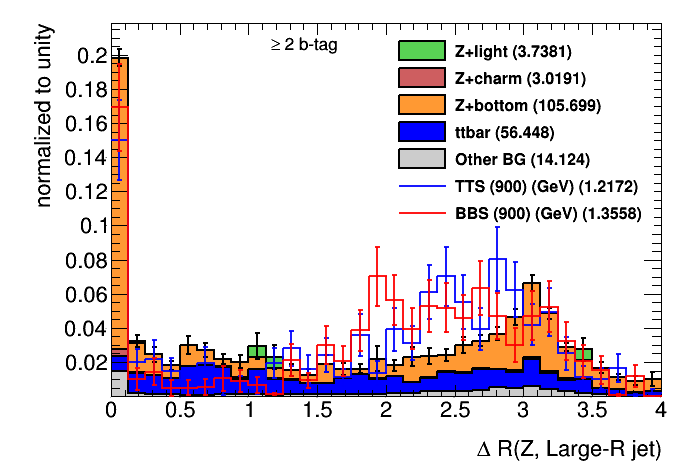
\includegraphics[width=10cm]{figures/deltaR.png}
\caption{Distribution for the $\Delta R$ of the large-R jets and the Z boson candidate after the preselection.}
\label{deltaR}
\end{figure}

      



\section{Basic Selection Implied by the Boosted WbZt Topology  }
The decay topologys TT \texorpdfstring{$\longrightarrow$}~ZtWb and BB \texorpdfstring{$\longrightarrow$}~ZbWt for the optimization studies in this analysis are defined as mentioned before. 
Because of the designated products of the vector-like quark decays further selection can be added to the preselection discussed in section \ref{Event preselection}, which is also used in more general studies without determining specific decay channels.       
It is reasonable that at least two large-R jets should be required considering that there is one top quark and one W boson, which could lead to large-R jets. 
Events without at least one top- and W-tag should also be rejected.  
Figure \ref{ljetmult} shows the multiplicity of the large-R jets.

\begin{figure}
\centering
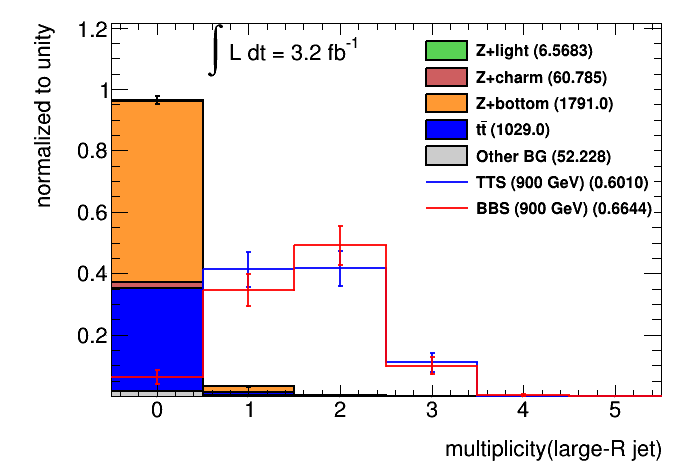
\includegraphics[width=10cm]{figures/multipliljet.png}
\caption{Plot for the large-R jet multiplicity after the preselection.}
\label{ljetmult}
\end{figure}

As expected the background processes mostly have no large-R jets because in most cases the $p_{T}$ of the particles is not high enough to produce large-R jets.
The decay topology considered in this analysis give reason to expect two large-R jets resulting from the boosted top Quark and W boson decays.
Therefore signal distribution looks not like expected caused by the fact that about 40 \% of the events only have one large-R jets. 
An explanation for the distribution could be, that the W bosons from T \texorpdfstring{$\longrightarrow$}~Wb and B \texorpdfstring{$\longrightarrow$}~Wt  could be located in an area of $\Delta R = 1.0$ around the Z candidate and therefore could be ignorated caused by the overlap removal mentioned earlier.
For the BBS signal process the case mentioned before is also possible for the jet resulting from the top quark.
Furthermore for the TTS signal process it is possible that the decay products of the W-boson and the top quark are clustered in one large-R jet because they are in an area of $\Delta R = 1.0$.\\
The requirement of two large-R jets selects the background from the signal and rejects a lot of background.
There are also a lot of signal events which are ignored because of the problematic mentioned before.
A representation for the distribution of the top- and W-tag multiplicity can be found in  figure \ref{topmultipli} and \ref{bosonmultipli}.

\newpage


\begin{figure}[h!]
\centering
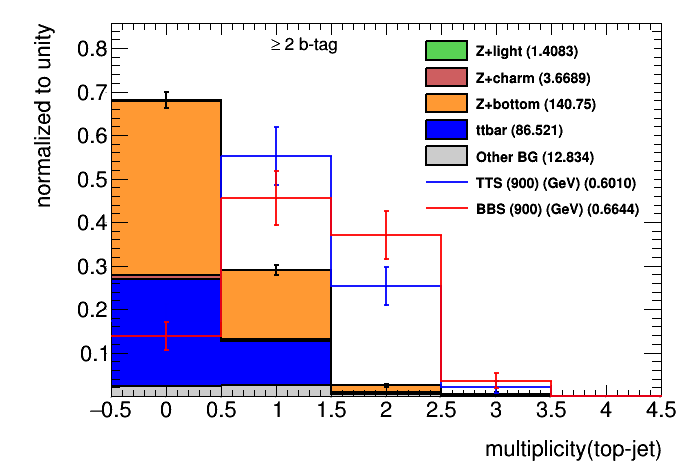
\includegraphics[width=11cm]{figures/topmultiplicity.png}
\caption{Plot for the top-tag multiplicity after the preselection.}
\label{topmultipli}
\end{figure}

\begin{figure}[h!]
\centering
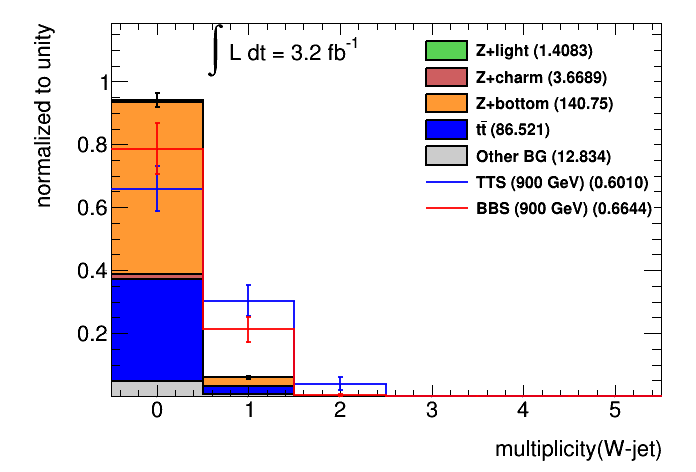
\includegraphics[width=11cm]{figures/Wmultiplicity.png}
\caption{Plot for the W-tag multiplicity after the preselection.}
\label{bosonmultipli}
\end{figure}

The plot for the top-tag multiplicity shows that most background events don't have a top-tagged large-R jet.
That is sensible if the Z+jets backgrounds are regarded because in these processes no top quark is included. 
The \ttbar{} process should also have no top-tag because the W bosons produced by the top quarks decay in the leptonic decay channel because there are two leptons required.
Therefore only  b-tagged jets are produced.
If the leptons resulting from the Z for the Z+jets backgrounds are not in an area $\Delta R = 1.0$ around the Z candidate they are not rejected by the overlap removal.
For the \ttbar{} process it is also possible that the leptons from the W boson decays are counted as large-R jets.
Hence there are some events with one top-tag in the background distribution.\\
The signal distribution looks not like assumed because there are a lot of events having two top-tagged large-R jets.
This is caused by the fact that the top-tagger also tag the large-R jet resulting from the W-boson as top-tag.\\
BEMERKUNG : vielleicht verteilung W-tagged jets die nicht getop-tagged sind in den Anhang zum aufzeigen?.\\
The background distribution for the W-tagged large-R jets can be explained with the same argumentation as for the top-tag multiplicity.
For the signal processes there is a high amount of events without W-tagged large-R jet ( about 80 \% for TTS and 65 \% for BBS), which is not like expected.
This could be caused by the argumentation mentioned before that the large-R jet pruduced by the W-boson is ignored because of the overlap removal.
In addition to that the boson-tagger doesn't work perfectly but has an efficiency of 50 \%.\\
After demanding all three parts of the basic selection implied by the boosted WbZt topology a lot of background is rejected which becomes obvious in the three discributions discribed before.
The unweighted number of events for signal and background after the basic selection is listed in table \ref{numberoevents}.
\vspace{-0.19cm}

\begin{table}
\centering
%\setlength{\tab}{\textwidth}
\begin{tabular}{|c|c|c|} 
\hline
\textbf{Process} & \textbf{Unweighted number of events} & \textbf{Weighted number of events}  \\
\hline
\hline
Z+light & 3 & 0.0005\\
Z+charm & 2 & 0.0060\\
Z+bottom & 77 & 0.1680\\
ttbar & 6 & 0.3739\\
Other BG & 1331 & 0.3298\\
TTS & 214 & 0.1094\\
BBS & 176 & 0.1089\\
\hline
\end{tabular}
\caption{Unweighted and weighted number of events for signal and background processes.}
\label{numberoevents}
\end{table}


The listed numbers reveal that after the event preselection and basic selection there are for both signal and background very  low numbers of events.
An optimization study without enough statistic is not convincing because the distributions are containing too much error.
Therefore the optimization study in this analysis is performed without requireing at least one W-tag.
The statistic after the basic selection is much higher for both signal and background without this requirement.

 


















